\documentclass[12pt,a4paper]{article}

\usepackage[slovak]{babel}
\usepackage[utf8]{inputenc}
\usepackage{listings}
\usepackage{graphicx}
\usepackage{tabularx} 
\usepackage{amsmath} 
\usepackage{amssymb} 

\lstset{
language=sh
,breaklines=true
,basicstyle=\ttfamily
, showstringspaces=false}

\author{Peter Csiba}
\textwidth 6.5in
\oddsidemargin 0.0in
\evensidemargin 0.0in

\title{Pravdepodobnostné metódy - Poznámky}
\date{19th of May, 2013}
\author{Peter Csiba, petherz@gmail.com}

\begin{document}
\maketitle


\section{Definície}

\subsection{Paštika} 
\begin{itemize} 
  \item cdf - cumulative distribution function $f(x) = Pr[X < x]$. 
  \item iid - independent and identically distributed random variables. 
  \item Markovova nerovnosť. Ak náhodná premenná $X$ nadobúda iba nezáporné hodnoty, tak $\forall k > 0 \, Pr[X \geq k] \leq E[x]/k$.
  \item Čebyševova nerovnosť $\forall k>0$ platí $Pr[|X-E[X]| \geq k] \leq Var[X]/k^2$. Dosadením do Markovovej nerovnosti. 
  \item Vyššie momenty. $Pr[(X-\mu)^m \geq t^m] \leq E[(X - \mu)^m]/t^m$. 
  \item Chernoff a Poissonove pokusy. $X_i$ sú iid nadobúdajúce 0,1. Potom platí $\forall \delta > 0 : Pr[X \geq (1 + \delta)\mu] < (e^\delta/(1 + \delta)^{(1+\delta)})^\mu$. Napr. pre hádzanie guličiek do krabíc získame pre $Pr[X \geq 2\mu]$ postupne $1/2$, $1/\mu$, $O(1/\mu^2)$ a Poissonove pokusy $e^{-\mu/3}$.
  \item Martingale. Postupnosť náhodných premenných $E[X_i | X_0, \ldots, X_{i-1}] = X_{i-1}$.
    \begin{itemize} 
      \item Bounded difference condition ak platí $|X_i - X_{i-1}| \leq c_i$.
      \item Azuma. Martingale $X$ tak $Pr[|X_n - X_0| > t] \leq 2 \exp{-t^2 / 2c}$ kde $c=\sum_i c_i^2$. TODO 
      \item Doobova postupnosť. Ak $X_i$ sú n.p. tak $Y_i = E_{X_{i+1}, \ldots, X_{n}}[f(X) | \overrightarrow{X_i}]$. TODO 
    \end{itemize} 
  \item (Weak) law of big numbers $lim_{n \Rightarrow \infty} Pr[|X - \mu| > \epsilon] = 0$. 
  \item Central limit theorem. $\sqrt{n}((\frac{1}{n}\sum_{i=1}^n X_i) - \mu)\ \rightarrow^d\ N(0,\;\sigma^2).$ 
  \item Randomizácia. Premena priemerného prípadu na očakávaný. Napr. pri hešovaní vyberieme náhodnú hešovaciu funkciu. 
  \item \emph{Perfektný zdroj náhodných bitov} je náhodná premenná, ktorej hodnotami sú nekonečné postupnosti $x_1, x_2, \ldots \in \{0,1\}^{*}$ bitov také, že
  $$
    \forall(y_1, \ldots, y_n) \in \{0,1\}^n \, Pr[x_i = y_i; i = 1,\ldots,n] = 2^{-n}
  $$ 
\end{itemize} 

\section{Pravdepodobnostné triky}
\begin{itemize} 
  \item Linearita strednej hodnoty $E[X + Y] = E[X] + E[Y]$. 
\end{itemize} 

\section{Ochutnávka pravdepodobnostných algoritmov}
pravdepodobnostné konečné automaty, testovanie násobenia matíc, hľadanie minimálneho rezu
   
Jeden z pohľadov na pp algoritmy: vieme medzi dvoma počítačmi vymieňať informácie iba draho a chceme skoro istú odpoveď. 
   
Ďalším delením modelov pp. alg: 
  \begin{itemize} 
    \item I. nederministicky vyberáme z deterministických stratégií. Algoritmy $S_{A,w} = \{A_1, \ldots, m\}$ a výpočty $C_i = A_i(w)$ so časovou zložitosťou $Time(C_i)$. Z toho odvodíme ExpTime, Time, výsledok $X$ a pp korektnosti $E[X]$. Napr. randomized max SAT. 
    \item II. simulujeme NTS. Napr. randomizovaný quicksort (keď je jeden z prvkov $i$,$j$ porovnaný - je vybraný ako pivot). 
  \end{itemize} 

  \subsection{Las Vegas a Monte Carlo} 
  \begin{itemize} 
    \item Las Vegas (LV). Keď odpovie, tak pravdivo, inak odpovie "nie som si istý". 
      \begin{itemize}
        \item $Pr[A(x) = F(x)] \geq 1/2$, 
        \item $Pr[A(x) = "?"] = 1 - Pr[A(x) = F(x)]$. 
      \end{itemize} 
      Táto definícia je ekvivalentná s $Pr[A(x) = F(x)] = 1$ a označuje sa LV* - ako potenciálne nekonečná.
      Napr. či $\exists i : a_i = b_i$. 
    \item Monte Carlo (MC). 
    \begin{itemize} 
      \item Jednosmerné (1MC) - istotu odmietne a možno (aspoň s pp 1/2) hovorí pravdu. Napr. porovnanie matíc. 
      \item S ohraničenou chybou (2MC) rátajúci funkciu $F(x)$ ak $$
        \exists 0 < \epsilon \leq 1/2 \, \forall x \, Prob[A(x) = F(x)] \geq 1/2 + \epsilon
      $$
      V tomto prípade opakovaním behu vyberieme najčastejšiu odpoveď, ktorá nastala aspon v $t/2$ prípadoch. 
      \item S {\bf ne}ohraničenou chybou (UMC) ak $Prob[A(x) = F(x)] > 1/2$. Prakticky 2MC s dynamickým parametrom $e_x$ ktorý môže byť exponenciálne malý od počtu vstupov čo vyžaduje exponenciálne veľa behov algoritmu pri opakovaní. V prípade $e_x = \frac{1}{log|x|}$ je to v pohode. Zaujímavosťou je, že v prípade "neviem" algoritmus vracia pravdepodobnosť "áno", t.j. zvyšných prípadov. 
    \end{itemize} 
    
    \item {\bf Izolačná lema 5.11} Nech $(X,F)$ je systém podmnožín rozmeru $m$, $w : X \mapsto \{1,\ldots,2m\}$ je kladná celočíselná váhovacia funkcia. Potom $Pr[\exists \mbox{jedina mnozina minimalnej vahy v} F] \geq 1/2$. Napr. perfektné párovanie - aby sme našli unikátne. 
  \end{itemize} 
  
  \subsection{Optimalizačné problémy} 
  Def: $U = (\Sigma_I, \Sigma_O, L, L_I, M, cena, ciel)$ kde 
  \begin{itemize}
    \item $\Sigma_I$ je vstupná abeceda.
    \item $\Sigma_O$ je výstupná abeceda.
    \item $L \subseteq \Sigma_I^{*}$ je jazyk prípustných vstupov.
    \item $L_I \subseteq L$ je jazyk aktuálnych vstupov.
    \item $M$ je jazyk potenciálnych riešení.
    \item $cena(x,M(x)) \in \mathbb{R}$ je účelová funkcia.
    \item $ciel \in \{min, max\}$.
    \item $OPT_U(x)$ je optimálne riešenie.
    \item Algoritmus $A$ je \emph{konzistentný} ak $A(x) \in M(x)$. 
    \item $Ratio_A(x) = max\{\frac{OPT(x)/A(x)}{A(x)/OPT(x)}\}$ - definícia kvôli rôznym cieľom. 
    \item $E[\delta]$-aproximačný ak $Prob[A(x) \in M(x)] = 1 \wedge \forall x \in L \, E[Ratio_A(x)] \leq \delta$. 
    \item $\delta$-aproximačný ak $Prob[A(x) \in M(x)] = 1 \wedge \forall x \in L \, Prob[Ratio_A(x) \leq \delta] \geq 1/2$. 
  \end{itemize} 
  
  {\bf Lema 2.4} Z Čebyševa dostávame, že ak $A$ je $E[\delta]$ aproximačný, tak je aj $2 \delta$ aproximačný. 
  
\subsection{Pravdepodobnostné zložitostné triedy}
\begin{figure}[H]
  \centering
  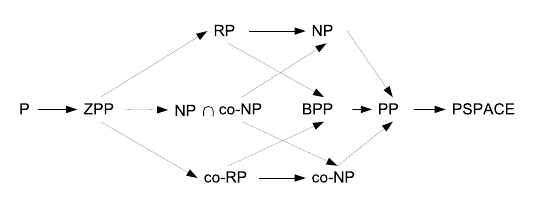
\includegraphics[width=0.9\textwidth]{hierarchy.png}
\end{figure}

\emph{Štandardizovaný TS} je NTS $M$: 
  \begin{itemize} 
    \item v každom kroku výpočtu má $M$ možnosť výberu z presne dvoch možností
    \item časová zložitosť $t(n)$ stroja $M$ je konštruovateľná
    \item každý výpočet stroja $M$ na vstupe $w$ je presne dĺžky $f(|w|)$ 
  \end{itemize}
  
\paragraph{Trieda Randomized Polynomial time (RP)}
Monte Carlo TS $M$ je štandardizovaný TS polynomiálnej časovej zložistosti, pre ktorý platí:  
\begin{itemize} 
  \item $w \in L \Rightarrow Pr[M(w) = accept] \geq 1/2$
  \item $w \not\in L \Rightarrow M(w) = reject$
\end{itemize}
Konštantu 1/2 môžeme nahradiť $0 < \epsilon < 1$ a opakovaným behom získame pôvodnú definíciu. Dokonca stačí polynomiálne ohraničenie: 
$$
x \in L \Rightarrow Prob[M(x) = 1] > \frac{1}{|q(|x|)|} \, \wedge \, x \not\in L \Rightarrow Prob[M(x) = 1] = 0
$$
Poznámka, v skriptách je $q(|x|)$, čo IMHO nestačí. A treba aj diskusiu ohľadom koreňov $q$.  

\paragraph{$P \subseteq RP \subseteq NP$.} 

\paragraph{co-RP} - naopak ako RP
\begin{itemize} 
  \item $w \in L \Rightarrow Pr[M(w) = reject] \geq 1/2$
  \item $w \not\in L \Rightarrow M(w) = accept$
\end{itemize}

\paragraph{ZPP} = $RP \cap co-RP$. 

\begin{figure}[H]
  \centering
  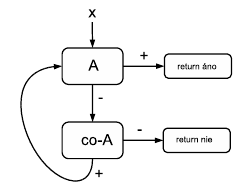
\includegraphics[width=0.4\textwidth]{zpp.png}
  \caption{ZPP je vlastne Las Vegas algoritmus (Veta 3.4 podľa obrázka).}
\end{figure}

\paragraph{PP.} Jazyk $L$ patrí do triedy $PP$ práve vtedy, ak existuje polynomiálne časovo ohraničený štandardizovaný $TS M$, pričom
$$
  w \in L \Leftrightarrow Pr[M(w) = accept] > 1/2
$$
Napr. $MAJ-CNF = \{F(x_1, \ldots, x_n) | \exists \mbox{aspon} 2^{n-1} (x_1,\ldots,x_n) \in \{0,1\}^n : F(x_1, \ldots, x_n) = 1\}$. 

\paragraph{$NP \subseteq PP \subseteq PSPACE$} V \emph{PSPACE} vieme simulovať \emph{PP}. Stroj \emph{PP} vie simulovať \emph{NP} tak, že si vyrobí polovicu výpočtov v ktorých akceptuje. 

Stále problém s \emph{exponenciálnym počtom opakovaní} v prípade, keď $\epsilon = 2^{-p(n)}$ kde $\epsilon$ je rozdiel $Pr[PP accept]$ a 1/2. 

\paragraph{BPP.} 
\begin{itemize} 
  \item ak $w \in L$ tak aspoň 3/4 výpočtov stroja $N$ sú akceptujúce 
  \item ak $w \not\in L$ tak aspoň 3/4 výpočtov stroja $N$ sú zamietajúce 
\end{itemize} 
TODO: Polynomiálny obvod? 

Veta 3.7. skip
Veta 3.8. skip 
Lema 3.9. skip  

\paragraph{$\delta-RP$}. Každá hrana pri rozhodovaní TS má pravdepodobnosti z intervalu $(\delta, 1-\delta)$. Platí $\delta-BPP = BPP$. TODO myšlienka dôkazu. 

\section{Analýza pravdepodobnostných algoritmov}
 - Markov, Čebyšev, Chernoff (aj s dôkazmi; v Chernoffovi stačí dokázať to najsilnejšie tvrdenie), vyššie momenty netreba
 
\paragraph{2-SAT-RandomWalk (Lema 3.11)} treba $n^2$ preklopení, dokazuje sa Čebyšovom cez $E[\mbox{preklopeni}]$. V prípade slabo-náhodného ($\delta$-náhodného) zdroja môže riešenie trvať exponenciálne dlho. 
 
 
\section{Metódy tvorby pravdepodobnostných algoritmov} 
\subsection{Eliminácia protihráča}
Myšlienka: náhodnou voľbou sa snažíme vyhnúť worst case-u, napr. výber pivota v quicksorte alebo prvočísla pri porovnaní databáz. 

TODO skip online algoritmy str. 44 - str. 49 

\subsection{Metóda svedkov}
Chceme zistiť, či $X$ má nejakú vlastnosť $V$. Odvodíme vlastnosti $W_i$, ktoré náhodne testujeme. Napr. test prvočíselnosti. 

\subsection{Metóda odtlačkov} 
Pri porovnaní objektov $X_1$ a $X_2$ porovnávame iba hodnoty $f(X_1)$ a $f(X_2)$. Je špeciálnym prípadom metódy svedkov. Napr. porovnanie dvoch súborov pomocou ich hashov, resp. prefixov. 

SKIP Interaktivne dokazy 4.2.4 str.56 - 57 (Krypto) 

Viď test prvočíselnosti \ref{sec:prime-test}. 

\subsubsection{Freivaldsova metóda}
Namiesto zvyšku po delení prvočíslom používame hodnotu polynómu, matice alebo funkcie. Napr. $AB=C$ pomocou náhodného vektoru $x$. Pri porovnaní polynómov môže byť normálny tvar exponenciálne dlhý, pričom zápis je lineárny $(x_1 + x_2)(x_1 + x_3) \cdots (x_2 + x_4)$. 
\paragraph{Schwartz-Zippel} Nech $Q(x_1, x_2, \ldots, x_n) \in F[x_1, x_2, \ldots, x_n]$ je polynóm viacerých premenných celkového stupňa $d$. Nech $S \subseteq F$ a $r_1, r_2, \ldots, r_n$ sú náhodne vybraté z $S$. Potom 
$$
  Pr[Q(r_1,\ldots,r_n) = 0 | Q(x_1, \ldots, x_n) \neq 0] \leq \frac{d}{|S|}
$$
Myšlienka dôkazu: maximálny počet rôznych koreňov polynómu nad $\mathbb{R}$ stupňa $d$ je $d$. Pre polynóm $Q(x_1, \ldots, x_n)$ nad $\mathbb{Z}_p$ je to $n \cdot d \cdot p^{n-1}$. Dôkaz: dvojrozmerná indukcia. 

\subsection{Random sampling} 
Náhodné hľadanie objektu generovaním. Derandomizácia prav. alg. 

Doteraz sme nezávislé opakovanie celých výpočtov využívali k znižovaniu chyby pod želanú hranicu. Metódu teraz potiahneme ďalej:
\begin{itemize} 
\item opakovanie nie celých výpočtov, ale len vybraných častí
\item opakovanie rôznych častí výpočtu rôzny počet krát: častejšie zopakujeme tie
časti, v ktorých je pravdepodobnosť výskytu chyby vyššia
\end{itemize} 
Viď Min-Cut \ref{sec:min-cut} 


\section{Triedenie a vyhľadávanie}
 - s.v.p. analýza quicksortu (dôkaz); treap, skiplist - vedieť, ako fungujú a myšlienky dôkazov
 

\section{Hľadanie mediánu}
 - algoritmus a jeho analýza
 

\section{Hešovanie}
 - univerzálne rodiny hešovacích funkcií (def.), perfektné hešovanie, lineárne sondovanie (aj s dôkazom očak. zložitosti)
 
Pre problém plánovania ukážeme, že pravdepodobnostný algoritmus dáva kvalitatívne lepšie riešenie ako ľubovoľný determinstický algoritmus.
 
\paragraph{Univerzálna trieda hešovacích funkcií}. Nech $H$ je konečná množina hešovacích funkcií $U \mapsto T = \{0,1,\ldots,m-1\}$. $H$ je univerzálna trieda funkcií, ak $\forall x,y \in U$, $x \neq y$ 
$$
  |\{h \in H | h(x) = h(y)\}| \leq \frac{|H|}{m}. 
$$
Napr. jednou triedou takých funkcií sú všetky funkcie $U \mapsto T$. Alebo $h_{a,b} = ((ax + b) \pmod p) \pmod m$ pre $U = \{0, 1, \ldots, p-1\}$. Alebo skalárny súčin pre $r$-rozmerné vektory. 

\section{Testovanie prvočíselnosti}
\label{sec:prime-test} 
 - Fermatov test (dôkaz Fermatovej vety, dôkaz, že ne-Carmichaelove zložené čísla majú veľa svedkov) a Miller-Rabinov test (ako funguje, že zložené čísla majú viac odmocnín z 1; dôkaz, že svedkov je veľa netreba)

(Metóda svedkov) 
Malá fermatová veta, O čínskych zvyškoch, Lagrangeova of grupách $|A| = |\{H \circ a | a \in H\}||H|$ kde $H$ je podgrupa $A$.  

\paragraph{Veta 4.29} Nech $p > 2$ je nepárne. Potom 
$$
  p \in \mathbb{P} \Leftrightarrow a^{\frac{p-1}{2}} \pmod p \in \{1, p-1\} \forall Z_p - \{0\}
$$

\paragraph{Algoritmus 21 - Zjednodušený Solovay-Strassen} je polytime 1MC algoritmus pre rozpoznávanie zložených čísel. 
\begin{itemize}
  \item náhodne $a \in \{1,\ldots,n-1\}$
  \item $A \Leftarrow a^{(n-1)/2} \pmod n$
  \item {\bf if} $A \in \{1, -1\}$ {\bf then} return($n \in \mathbb{P}$)
  \item {\bf else} return($n \not\in \mathbb{P}$)
\end{itemize} 
Rozšírený používa {\bf Jakobián} $n \geq 3$ je nepárne, potom $a \in \{1,\ldots,n-1\}$ je {\bf Jac-svedok} pre $n \not\in PRIM$, ak 
\begin{itemize} 
  \item $gcd(a,n) \neq 1$, alebo
  \item $gcd(a,n) = 1$ a $Jac[\frac{a}{n}] \neq a^{(n-1)/2} \pmod n$
\end{itemize} 
TODO co je Jakobian 

\paragraph{PrimGen($l$,$k$)}. Opakujeme $l^2$ krát vygenerujeme $l$ bitové číslo a $k$-krát naň spustíme Solovay-Strassen. Zaujímavosťou je, že zložitosť počítame vzhľadom na veľkosť výstupu. 

\section{Konvexné obaly (a veľa iného)}
 - randomizovaný inkrementálny algoritmus pre konvexný obal v 2D a spätná analýza; pre viacrozmerný KO a súvis s Delaunayho trianguláciou, Voronoiovym diagramom stačí myšlienku, dôkaz netreba
 

\section{Lineárne programovanie}
 - Seidelov algoritmus (aj s dôkazom zložitosti), MSW a Clarksonove algoritmy vedieť ako fungujú, dôkaz netreba
 
\paragraph{Definícia 4.8} 
\begin{itemize} 
  \item vstup matica $A = [a_{ij}]$, $i = 1,\ldots,m$; $j=1,\ldots,n$
  \item vstup vektor $b \in \mathbb{R}^m$
  \item vstup vektor $c \in \mathbb{R}^n$
  \item ohraničenia $M(A,b,c) = \{X \in (\mathbb{R}^{0,+} | AX = b\}$
  \item cena $cost(X, (A,b,c)) = c^TX = \sum_i c_ix_i$
  \item cieľom je minimalizácia ceny pri dodržaní ohraničení
\end{itemize} 
Pre obor hodnôt riešení $X$, ak je $\mathbb{R}$ tak existuje polynomiálny algoritmus, ak je $\mathbb{Z}$ (integer LP = ILP)( tak je exponenciálny. Preto existuje trieda aproximačných algoritmov, ktoré najprv zrelaxujú problém na $\mathbb{R}$, vyriešia v polytime a transformujú na prípustné riešenie pôvodného problému. Používa sa napr. {\bf náhodné zaokrúhľovanie}. 

Demonštrácia na probléme {\bf vrcholového pokrytia}. Minimalizovať $\sum_i x_i$ pričom $x_i + x_j \geq 1 \forall (v_i, v_j) \in E$. Vzniká tak 2-aproximačný algoritmus. 

Podobným spôsobom vieme aproximovať aj MaxSAT v polynomiálnom čase a $E[\frac{e}{e-1}]$ aproximáciou. TODO dôkaz. 

\section{Hľadanie minimálneho rezu}
\label{sec:min-cut} 
 - jednoduchý kontrahovací algoritmus a jeho zrýchlenia; sparsifikátory len myšlienku, vedieť čo to je, na čo to je...
 
Vstup: ohodnotený graf (nezápornými číslami). Algoritmus: kým viac ako dva vrcholy, tak náhodne vyber hranu (vyššia cena, vyššia pp) a skontrahuj; výsledkom sú hrany medzi $C_1$ a $C_2$. Analýza: beh $O(n^2)$ lebo $n$-krát kontrahujeme maximálne $n$ hrán. Úspešnosť $\frac{2}{n(n-1)}$, lebo minimálna cena rezu dáva dolný odhad na minimálny váhovaný stupeň vrchola. 

TODO dôkaz 

Zlepšíme tak, že po $l(n)$ krokoch kontrakciu zastavíme a dopočítame deterministicky. 
\paragraph{Veta 4.20} Algoritmus $DetRan(n^{2/3})$ (pre $l(n) = n^{2/3}$) opakovaný $\frac{n^2}{l^2(n)} = n^{4/3}$-krát vypočíta v čase $O(\frac{n^4}{l^2(n)}) = O(n^{8/3})$ minimálny rez s pravdepodobnosťou úspechu aspoň $1 - \frac{1}{e}$. 

\paragraph{Veta 4.21} Časová zložitosť algoritmu $RepTree$ je $O(n^logn)$ s pravdepodobnosťou úspechu aspoň $\frac{1}{\Theta(log n)}$. Algoritmus paralelne simuluje opakované behy pôvodného kontrakčného algoritmuk pričom sa vetví, t.j. vytvorí dve rôzne kontrakcie a tak počet simulácií zdvojnásobí, vždy po $1 + \frac{n}{\sqrt{2}}$ krokoch.  

TODO dôkaz. 

Dá sa nejak aj pomocou semidefinitného programovania (SKIP 4.6.). 

\section{Hľadanie najlacnejšej kostry}
 - lineárny samplovací algoritmus pre hľadanie najlacnejšej kostry
 

\section{Perfektné párovania}
 - perfektné párovania, Tutteova veta (aj dôkaz), testovanie rovnosti polynómov, Schwartz-Zippelova lema (aj dôkaz), izolačná lema (aj dôkaz)
 
\paragraph{Edmondson} Nech $A$ je matica typu $n \times n$, ktorú k bipartitnému grafu $G(U,V,E)$ skonštruujeme nasledovne
\begin{align*} 
A[i,j] = \left\{ 
  \begin{array}{ll}
    x_{ij}, & (u_i, v_j) \in E \\
    0, & (u_i, v_j) \not\in E \\
  \end{array} 
\right.
\end{align*} 
Definujeme polynóm $Q(x_{11}, \ldots, x_{nn}) = det(A)$. Potom $G$ má úplne párovanie práve vtedy ak $Q \not\equiv 0$. 

\paragraph{Veta 5.9 Tutte} Nech $A$ je matica, ktorá vznikla z grafu $G = (V,E)$: 
\begin{itemize} 
  \item každej hrane $(v_i, v_j) \in E$ priradíme premennú $x_{i,j}$, $i < j$
  \item hodnota matice je 0 ak tam nie je hrana, $x_{i,j}$ ak $i < j$ a $-x_{i,j}$ ak $j < i$. 
\end{itemize} 
Potom $G$ obsahuje úplné párovanie práve vtedy, keď determinant matice $A$ je nenulový. 
TODO RNC algoritmus. 

\paragraph{P-Match} Existuje podmienka pre hranu, či je súčasťou perfektného párovania (je závislá od determinantu upravenej Tutteho matice $x_{i,j} \mapsto 2^{w(i,j)}$. Tento algoritmus potrebuje $O(log^2n$ paralelné a $O(n^{3.5}m)$ práce. 

\section{Hľadanie najkratších ciest}
 - Seidelov algoritmus a hľadanie svedkov Booleovského násobenia matíc
 

\section{Náhodné prechádzky}
 - def. Markovove reťazce, prechodové matice a stacionárne distribúcie; hlavná veta MR (bez dôkazu); súvis s vlastnými číslami, súvis s elektrinou (efektívny odpor a "pendlovací čas", horný a dolný odhad pre čas pokrytia - aj s dôkazmi)
 

\section{Problém splniteľnosti}
 - Schöningov algoritmus na riešenie 3-SATu (aj s dôkazom zložitosti)
 
(Zvýšenie úspešnosti opakovaním a náhodná vzorka) 
\paragraph{Schoning}
\begin{itemize} 
  \item opakuj $S = 20 \cdot \sqrt{3\pi n}(\frac{4}{3})^n$-krát
  \item vygeneruj náhodný binárny vektor $\alpha$
  \item $\forall \alpha:$ RandomWalk $3n$-krát, zmeň náhodný bit v nesplnenej klauzule
\end{itemize} 
TODO seriously mame vediet dokaz?! (str. 65) 
Myšlienka: Nech $\alpha^{*}$ je splnený vektor a nech $x \in C(j)$ sú vektory s $Dist(\alpha^{*}, x) = j$. Pravdepodobnosť, že sa priblížime je $1/3$ a že oddialime je $2/3$. Vyhovujúcich postuností je
$$
  \binom{j + 2i - 1}{i} - \binom{j + 2i - 1}{i - 1} = \binom{j + 2i}{i}\frac{1}{j + 2i}
$$
kde $i$ je počet oddialení a $j$ počet priblížení (Pripomína Catalanove čísla). Už nám len stačí zrátať sumu cez $i$ a využiť Stirlingovu formulu $r! \approx \sqrt{2\pi r}(\frac{r}{e})^r$. 

Dá sa aj pomocou relaxácie ILP. 

Keďže máme viacero algoritmov na riešenie MaxSAT, tak sa ich oplatí skombinovať a zobrať lepší výsledok. Konkrétne RSAM (náhodný vektor a jeho okolie) a RRR (relaxácia ILP) a dostaneme tak $E[4/3]$-aproximačný algoritmus. TODO dôkaz. 

\section{Markov Chain Monte Carlo (MCMC)}
 - samplovanie pomocou náhodných prechádzok (náhodné grafy s predpísanými stupňami, náhodné riešenia knapsacku), reverzibilné MR a Metropolisov-Hastingsov algoritmus (ako vyrobiť MR s danou stacionárnou distribúciou); bayesovská inferencia a MrBayes (myšlienka)
 

\section{Náhodnosť a zložitosť}
 - pravdepodobnostné triedy zložitosti (ZPP, RP, coRP, BPP, PP), Adlemanova veta (BPP a boolovské obvody), Sipser-Gacsova veta (BPP a polynomiálna hierarchia)
 
 
SKIP: Paralelne a distribuovane vypocty 

\section{Arturove Merlinove hry}
 - triedy MA a AM, protokol pre grafový neizomorfizmus so súkromnou a verejnou mincou (t.j. GNI je v IP[2] aj v AM), protokoly v MA a AM sa dajú upraviť tak, aby mali perfektnú úplnosť; zosilnenie Sipser-Gacsovej vety: $MA \subseteq \Sigma 2P$; $MA \subseteq AM \subseteq \Pi 2P$
 

\section{Interaktívne dôkazy}
 - \# $P \subseteq IP \subseteq PSPACE$; myšlienka $IP = PSPACE$
 

\section{Pravdepodobnostne overiteľné dôkazy}
 - NP = PCP[n3, 1] (dôkaz)
 

\section{Derandomizácia} 
- derandomizácia pomocou pseudonáhodných generátorov (kap. 20.1. z Aroru); Nisan-Wigdersonov generátor (ako funguje, čo sú dizajny; dôkaz netreba)

\section{Ostatné}
Problém koordinácie - každý procesor chce načítať rovnakú hodnotu "*". Deterministické riešenie $O(n^{1/3})$ (TODO nechápem ako môže byť menej ako $O(n)$). Pravdepodobnostné konštantné s pravdepodobnosťou $1 - 2^{\Theta(c)}$. Podobne sa dá zlepšiť problém byzantíjskej dohody, kde sa procesory môžu správať náhodne (avšak to vyžaduje prídavný register s global read a synchronizáciu, ktorý náhodne generuje bity). 

TODO dôkazy a definície

TODO voľba šéfa

TODO section 5.2 - Formálne jazyky a automaty 



\end{document}

